\PassOptionsToPackage{unicode=true}{hyperref} % options for packages loaded elsewhere
\PassOptionsToPackage{hyphens}{url}
%
\documentclass[
  10pt,
  ignorenonframetext,
]{beamer}
\usepackage{pgfpages}
\setbeamertemplate{caption}[numbered]
\setbeamertemplate{caption label separator}{: }
\setbeamercolor{caption name}{fg=normal text.fg}
\beamertemplatenavigationsymbolsempty
% Prevent slide breaks in the middle of a paragraph:
\widowpenalties 1 10000
\raggedbottom
\setbeamertemplate{part page}{
  \centering
  \begin{beamercolorbox}[sep=16pt,center]{part title}
    \usebeamerfont{part title}\insertpart\par
  \end{beamercolorbox}
}
\setbeamertemplate{section page}{
  \centering
  \begin{beamercolorbox}[sep=12pt,center]{part title}
    \usebeamerfont{section title}\insertsection\par
  \end{beamercolorbox}
}
\setbeamertemplate{subsection page}{
  \centering
  \begin{beamercolorbox}[sep=8pt,center]{part title}
    \usebeamerfont{subsection title}\insertsubsection\par
  \end{beamercolorbox}
}
\AtBeginPart{
  \frame{\partpage}
}
\AtBeginSection{
  \ifbibliography
  \else
    \frame{\sectionpage}
  \fi
}
\AtBeginSubsection{
  \frame{\subsectionpage}
}
\usepackage{lmodern}
\usepackage{amssymb,amsmath}
\usepackage{ifxetex,ifluatex}
\ifnum 0\ifxetex 1\fi\ifluatex 1\fi=0 % if pdftex
  \usepackage[T1]{fontenc}
  \usepackage[utf8]{inputenc}
  \usepackage{textcomp} % provides euro and other symbols
\else % if luatex or xelatex
  \usepackage{unicode-math}
  \defaultfontfeatures{Scale=MatchLowercase}
  \defaultfontfeatures[\rmfamily]{Ligatures=TeX,Scale=1}
\fi
\usetheme[]{Dresden}
\usecolortheme{dolphin}
\usefonttheme{structuresmallcapsserif}
% use upquote if available, for straight quotes in verbatim environments
\IfFileExists{upquote.sty}{\usepackage{upquote}}{}
\IfFileExists{microtype.sty}{% use microtype if available
  \usepackage[]{microtype}
  \UseMicrotypeSet[protrusion]{basicmath} % disable protrusion for tt fonts
}{}
\makeatletter
\@ifundefined{KOMAClassName}{% if non-KOMA class
  \IfFileExists{parskip.sty}{%
    \usepackage{parskip}
  }{% else
    \setlength{\parindent}{0pt}
    \setlength{\parskip}{6pt plus 2pt minus 1pt}}
}{% if KOMA class
  \KOMAoptions{parskip=half}}
\makeatother
\usepackage{xcolor}
\IfFileExists{xurl.sty}{\usepackage{xurl}}{} % add URL line breaks if available
\IfFileExists{bookmark.sty}{\usepackage{bookmark}}{\usepackage{hyperref}}
\hypersetup{
  pdftitle={Random Forests},
  pdfauthor={Jan-Philipp Kolb},
  pdfborder={0 0 0},
  breaklinks=true}
\urlstyle{same}  % don't use monospace font for urls
\newif\ifbibliography
\usepackage{color}
\usepackage{fancyvrb}
\newcommand{\VerbBar}{|}
\newcommand{\VERB}{\Verb[commandchars=\\\{\}]}
\DefineVerbatimEnvironment{Highlighting}{Verbatim}{commandchars=\\\{\}}
% Add ',fontsize=\small' for more characters per line
\newenvironment{Shaded}{}{}
\newcommand{\AlertTok}[1]{\textcolor[rgb]{1.00,0.00,0.00}{#1}}
\newcommand{\AnnotationTok}[1]{\textcolor[rgb]{0.00,0.50,0.00}{#1}}
\newcommand{\AttributeTok}[1]{#1}
\newcommand{\BaseNTok}[1]{#1}
\newcommand{\BuiltInTok}[1]{#1}
\newcommand{\CharTok}[1]{\textcolor[rgb]{0.00,0.50,0.50}{#1}}
\newcommand{\CommentTok}[1]{\textcolor[rgb]{0.00,0.50,0.00}{#1}}
\newcommand{\CommentVarTok}[1]{\textcolor[rgb]{0.00,0.50,0.00}{#1}}
\newcommand{\ConstantTok}[1]{#1}
\newcommand{\ControlFlowTok}[1]{\textcolor[rgb]{0.00,0.00,1.00}{#1}}
\newcommand{\DataTypeTok}[1]{#1}
\newcommand{\DecValTok}[1]{#1}
\newcommand{\DocumentationTok}[1]{\textcolor[rgb]{0.00,0.50,0.00}{#1}}
\newcommand{\ErrorTok}[1]{\textcolor[rgb]{1.00,0.00,0.00}{\textbf{#1}}}
\newcommand{\ExtensionTok}[1]{#1}
\newcommand{\FloatTok}[1]{#1}
\newcommand{\FunctionTok}[1]{#1}
\newcommand{\ImportTok}[1]{#1}
\newcommand{\InformationTok}[1]{\textcolor[rgb]{0.00,0.50,0.00}{#1}}
\newcommand{\KeywordTok}[1]{\textcolor[rgb]{0.00,0.00,1.00}{#1}}
\newcommand{\NormalTok}[1]{#1}
\newcommand{\OperatorTok}[1]{#1}
\newcommand{\OtherTok}[1]{\textcolor[rgb]{1.00,0.25,0.00}{#1}}
\newcommand{\PreprocessorTok}[1]{\textcolor[rgb]{1.00,0.25,0.00}{#1}}
\newcommand{\RegionMarkerTok}[1]{#1}
\newcommand{\SpecialCharTok}[1]{\textcolor[rgb]{0.00,0.50,0.50}{#1}}
\newcommand{\SpecialStringTok}[1]{\textcolor[rgb]{0.00,0.50,0.50}{#1}}
\newcommand{\StringTok}[1]{\textcolor[rgb]{0.00,0.50,0.50}{#1}}
\newcommand{\VariableTok}[1]{#1}
\newcommand{\VerbatimStringTok}[1]{\textcolor[rgb]{0.00,0.50,0.50}{#1}}
\newcommand{\WarningTok}[1]{\textcolor[rgb]{0.00,0.50,0.00}{\textbf{#1}}}
\usepackage{graphicx,grffile}
\makeatletter
\def\maxwidth{\ifdim\Gin@nat@width>\linewidth\linewidth\else\Gin@nat@width\fi}
\def\maxheight{\ifdim\Gin@nat@height>\textheight\textheight\else\Gin@nat@height\fi}
\makeatother
% Scale images if necessary, so that they will not overflow the page
% margins by default, and it is still possible to overwrite the defaults
% using explicit options in \includegraphics[width, height, ...]{}
\setkeys{Gin}{width=\maxwidth,height=\maxheight,keepaspectratio}
\setlength{\emergencystretch}{3em}  % prevent overfull lines
\providecommand{\tightlist}{%
  \setlength{\itemsep}{0pt}\setlength{\parskip}{0pt}}
\setcounter{secnumdepth}{-2}

% set default figure placement to htbp
\makeatletter
\def\fps@figure{htbp}
\makeatother


\title{Random Forests}
\author{Jan-Philipp Kolb}
\date{04 Juni, 2019}

\begin{document}
\frame{\titlepage}

\begin{frame}{Random Forests}
\protect\hypertarget{random-forests}{}

\begin{itemize}
\tightlist
\item
  \href{https://en.wikipedia.org/wiki/Bootstrap_aggregating}{\textbf{Bagging}}
  can turn a single tree model with high variance and poor predictive
  power into a fairly accurate prediction function.
\item
  But bagging suffers from
  \href{https://stats.stackexchange.com/questions/295868/why-is-tree-correlation-a-problem-when-working-with-bagging}{\textbf{tree
  correlation}}, which reduces the overall performance of the model.
\item
  \href{https://en.wikipedia.org/wiki/Random_forest}{\textbf{Random
  forests}} are a modification of bagging that builds a large collection
  of de-correlated trees
\item
  It is a very popular
  \href{https://en.wikipedia.org/wiki/Out_of_the_box_(feature)}{\textbf{out-of-the-box}}
  learning algorithm that enjoys good predictive performance.
\end{itemize}

\end{frame}

\begin{frame}{Extending the bagging technique}
\protect\hypertarget{extending-the-bagging-technique}{}

\begin{itemize}
\tightlist
\item
  Bagging introduces a random component in to the tree building process 
\item
  The trees in bagging are not completely independent of each other
  since all the original predictors are considered at every split of
  every tree.
\item
  Trees from different bootstrap samples have similar structure to each
  other (especially at the top of the tree) due to underlying
  relationships.
\end{itemize}

\end{frame}

\begin{frame}[fragile]{Similar trees - tree correlation}
\protect\hypertarget{similar-trees---tree-correlation}{}

\begin{itemize}
\tightlist
\item
  If we create six decision trees with different bootstrapped samples of
  the Boston housing data, the top of the trees all have a very similar
  structure.
\item
  Although there are 15 predictor variables to split on, all six trees
  have both \texttt{lstat} and \texttt{rm} variables driving the first
  few splits.
\end{itemize}

\begin{figure}
\centering
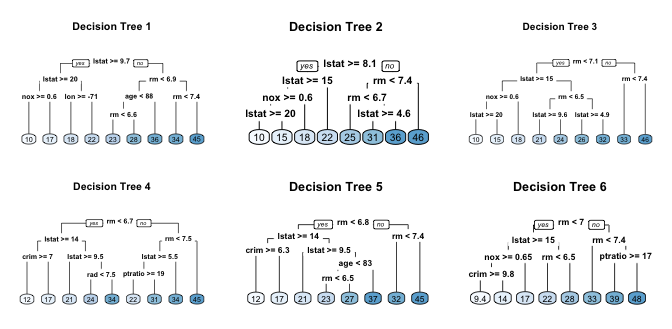
\includegraphics{figure/tree-correlation-1.png}
\caption{Six decision trees based on different bootstrap samples.}
\end{figure}

\end{frame}

\begin{frame}{Tree correlation}
\protect\hypertarget{tree-correlation}{}

\begin{itemize}
\tightlist
\item
  Tree correlation prevents bagging from optimally reducing variance of
  the predictive values.
\item
  To reduce variance further, we need to minimize the amount of
  correlation between the trees.
\item
  This can be achieved by injecting more randomness into the
  tree-growing process.
\end{itemize}

\end{frame}

\begin{frame}{Random forests achieve this in two ways:}
\protect\hypertarget{random-forests-achieve-this-in-two-ways}{}

\begin{enumerate}
[1)]
\tightlist
\item
  Bootstrap:
\end{enumerate}

\begin{itemize}
\tightlist
\item
  Similar to bagging, each tree is grown to a bootstrap resampled data
  set, which makes them different and decorrelates them.
\end{itemize}

\begin{enumerate}
[1)]
\setcounter{enumi}{1}
\tightlist
\item
  Split-variable randomization:
\end{enumerate}

\begin{itemize}
\tightlist
\item
  For every split, the search for the split variable is limited to a
  random subset of \(m\) of the \(p\) variables. 
\item
  For regression trees, typical default values are \(m=p/3\) (tuning
  parameter).
\item
  When \(m=p\), the randomization is limited (only step 1) and is the
  same as bagging.
\end{itemize}

\end{frame}

\begin{frame}[fragile]{Basic algorithm}
\protect\hypertarget{basic-algorithm}{}

The basic algorithm for a regression random forest can be generalized:

\begin{verbatim}
1.  Given training data set
2.  Select number of trees to build (ntrees)
3.  for i = 1 to ntrees do
4.  |  Generate a bootstrap sample of the original data
5.  |  Grow a regression tree to the bootstrapped data
6.  |  for each split do
7.  |  | Select m variables at random from all p variables
8.  |  | Pick the best variable/split-point among the m
9.  |  | Split the node into two child nodes
10. |  end
11. | Use tree model stopping criteria to determine: tree complete 
12. end
\end{verbatim}

The algorithm randomly selects a bootstrap sample to train and
predictors to use at each split.

\end{frame}

\begin{frame}{Characteristics}
\protect\hypertarget{characteristics}{}

\begin{itemize}
\tightlist
\item
  Since bootstrap samples and features are selected randomly at each
  split, we create a more diverse set of trees, which tends to lessen
  tree correlation beyond bagged trees and often dramatically increase
  predictive power. 
\end{itemize}

\begin{block}{out-of-bag error}

\begin{itemize}
\tightlist
\item
  Similar to bagging, a natural benefit of the bootstrap resampling
  process is that random forests have an
  \href{https://en.wikipedia.org/wiki/Out-of-bag_error}{\textbf{out-of-bag}}
  (OOB) sample that provides an efficient and reasonable approximation
  of the test error.
\item
  This provides a built-in validation set without any extra work, and
  you do not need to sacrifice any of your training data to use for
  validation.
\item
  We are more efficient identifying the number of trees required to
  stablize the error rate 
\end{itemize}

\end{block}

\end{frame}

\begin{frame}[fragile]{Preparation - random forests}
\protect\hypertarget{preparation---random-forests}{}

\begin{itemize}
\tightlist
\item
  The following slides are based on UC Business Analytics R Programming
  Guide on \href{http://uc-r.github.io/random_forests}{\textbf{random
  forests}}
\end{itemize}

\begin{Shaded}
\begin{Highlighting}[]
\KeywordTok{library}\NormalTok{(rsample)      }\CommentTok{# data splitting }
\KeywordTok{library}\NormalTok{(randomForest) }\CommentTok{# basic implementation}
\KeywordTok{library}\NormalTok{(ranger)       }\CommentTok{# a faster implementation of randomForest}
\CommentTok{# an aggregator package for performing many }
\CommentTok{# machine learning models}
\KeywordTok{library}\NormalTok{(caret)        }
\end{Highlighting}
\end{Shaded}

\end{frame}

\begin{frame}[fragile]{The Ames housing data}
\protect\hypertarget{the-ames-housing-data}{}

\begin{Shaded}
\begin{Highlighting}[]
\KeywordTok{set.seed}\NormalTok{(}\DecValTok{123}\NormalTok{)}
\NormalTok{ames_data <-}\StringTok{ }\NormalTok{AmesHousing}\OperatorTok{::}\NormalTok{ames_raw}
\end{Highlighting}
\end{Shaded}

\begin{Shaded}
\begin{Highlighting}[]
\KeywordTok{set.seed}\NormalTok{(}\DecValTok{123}\NormalTok{)}
\NormalTok{ames_split <-}\StringTok{ }\NormalTok{rsample}\OperatorTok{::}\KeywordTok{initial_split}\NormalTok{(ames_data,}\DataTypeTok{prop=}\NormalTok{.}\DecValTok{7}\NormalTok{)}
\NormalTok{ames_train <-}\StringTok{ }\NormalTok{rsample}\OperatorTok{::}\KeywordTok{training}\NormalTok{(ames_split)}
\NormalTok{ames_test  <-}\StringTok{ }\NormalTok{rsample}\OperatorTok{::}\KeywordTok{testing}\NormalTok{(ames_split)}
\end{Highlighting}
\end{Shaded}

\end{frame}

\begin{frame}[fragile]{Basic implementation}
\protect\hypertarget{basic-implementation}{}

\begin{itemize}
\tightlist
\item
  There are over 20 random forest packages in R.
\item
  To demonstrate the basic implementation we use the
  \texttt{randomForest} package, the oldest and most well known
  implementation of the random forest algorithm in R.
\item
  As your data set grows in size \texttt{randomForest} does not scale
  well (although you can parallelize with \texttt{foreach}).
\item
  To explore and compare a variety of tuning parameters we can find more
  effective packages.
\item
  The package \texttt{ranger} will be presented in the tuning section.
\end{itemize}

\end{frame}

\begin{frame}[fragile]{\texttt{randomForest::randomForest}}
\protect\hypertarget{randomforestrandomforest}{}

\begin{itemize}
\tightlist
\item
  \texttt{randomForest} can use the formula or x-y matrix notation.
\item
  Below we apply the default \texttt{randomForest} model using the
  formal specification.
\item
  The default random forest performs 500 trees and
  \(\dfrac{\text{nr. features}}{3}=26\) randomly selected predictor
  variables at each split.
\end{itemize}

\begin{Shaded}
\begin{Highlighting}[]
\KeywordTok{set.seed}\NormalTok{(}\DecValTok{123}\NormalTok{)}
\CommentTok{# default RF model}
\NormalTok{(m1 <-}\StringTok{ }\KeywordTok{randomForest}\NormalTok{(}\DataTypeTok{formula =}\NormalTok{ Sale_Price }\OperatorTok{~}\StringTok{ }\NormalTok{.,}\DataTypeTok{data=}\NormalTok{ames_train))}
\end{Highlighting}
\end{Shaded}

\begin{verbatim}
## 
## Call:
##  randomForest(formula = Sale_Price ~ ., data = ames_train) 
##                Type of random forest: regression
##                      Number of trees: 500
## No. of variables tried at each split: 26
## 
##           Mean of squared residuals: 639516350
##                     % Var explained: 89.7
\end{verbatim}

\end{frame}

\begin{frame}[fragile]{Plotting the model}
\protect\hypertarget{plotting-the-model}{}

\begin{itemize}
\tightlist
\item
  The error rate stabalizes with around 100 trees but continues to
  decrease slowly until around 300 trees.
\end{itemize}

\begin{Shaded}
\begin{Highlighting}[]
\KeywordTok{plot}\NormalTok{(m1,}\DataTypeTok{main=}\StringTok{"Error rate"}\NormalTok{)}
\end{Highlighting}
\end{Shaded}

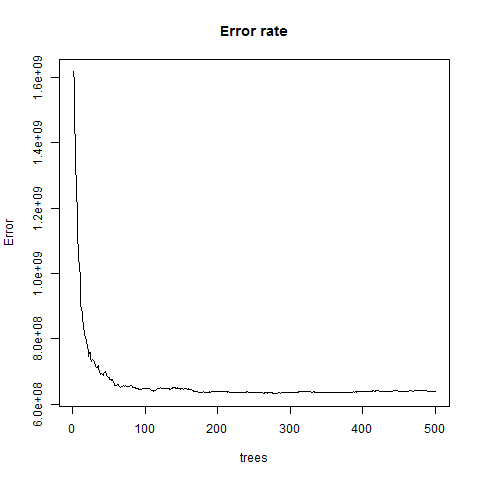
\includegraphics[width=\textwidth,height=0.65\textheight]{figure/ml_rf_errorrate_m1.png}

\end{frame}

\begin{frame}{Random forests - out-of-the-box algorithm}
\protect\hypertarget{random-forests---out-of-the-box-algorithm}{}

\begin{itemize}
\tightlist
\item
  Random forests perform remarkably well with very little tuning.
\item
  We get an RMSE of less than 30K dollar without any tuning.
\item
  This is more than 6K dollar RMSE-reduction compared to a fully-tuned
  bagging model
\item
  and 4K dollar reduction to to a fully-tuned elastic net model.
\item
  We can still seek improvement by tuning our random forest model.
\end{itemize}

\begin{block}{Tuning Random forests}

\begin{itemize}
\tightlist
\item
  Random forests are fairly easy to tune since there are only a handful
  of tuning parameters.
\item
  First we tune the number of candidate variables to select from at each
  split.
\item
  A few additional hyperparameters are important.
\end{itemize}

\end{block}

\end{frame}

\begin{frame}[fragile]{Tuning parameters (I)}
\protect\hypertarget{tuning-parameters-i}{}

\begin{itemize}
\tightlist
\item
  The following hyperparameter are important (names may differ across
  packages):
\end{itemize}

\begin{block}{number of trees}

\begin{itemize}
\tightlist
\item
  \texttt{ntree} - We want enough trees to stabalize the error but using
  too many trees is inefficient, esp.~for large data sets.
\end{itemize}

\end{block}

\begin{block}{number of variables}

\begin{itemize}
\tightlist
\item
  \texttt{mtry} - number of variables as candidates at each split. When
  \texttt{mtry=p} the model equates to bagging.
\item
  When \texttt{mtry=1} the split variable is completely random, all
  variables get a chance but can lead to biased results. Suggestion:
  start with 5 values evenly spaced across the range from 2 to p.
\end{itemize}

\end{block}

\end{frame}

\begin{frame}[fragile]{Tuning parameters (II)}
\protect\hypertarget{tuning-parameters-ii}{}

\begin{block}{Number of samples}

\begin{itemize}
\tightlist
\item
  \texttt{sampsize} - Default value is 63.25\% since this is the
  expected value of unique observations in the bootstrap sample.
\item
  Lower sample sizes can reduce training time but may introduce more
  bias. Increasing sample size can increase performance but at risk of
  overfitting - it introduces more variance. 
\end{itemize}

\end{block}

\end{frame}

\begin{frame}[fragile]{Tuning parameters (III)}
\protect\hypertarget{tuning-parameters-iii}{}

\begin{block}{minimum number of samples within the terminal nodes:}

\begin{itemize}
\tightlist
\item
  \texttt{nodesize} - Controls the complexity of the trees.
\item
  It is the minimum size of terminal nodes.
\item
  Smaller node size allow for deeper, more complex trees
\item
  This is another bias-variance tradeoff where deeper trees introduce
  more variance (risk of overfitting)
\item
  Shallower trees introduce more bias (risk of not fully capturing
  unique patters and relatonships in the data).
\end{itemize}

\end{block}

\begin{block}{maximum number of terminal nodes}

\begin{itemize}
\tightlist
\item
  \texttt{maxnodes}: A way to control the complexity of the trees.
\item
  More nodes equates to deeper, more complex trees.
\item
  Less nodes result in shallower trees.
\end{itemize}

\end{block}

\end{frame}

\begin{frame}[fragile]{Initial tuning with \texttt{randomForest}}
\protect\hypertarget{initial-tuning-with-randomforest}{}

\begin{itemize}
\tightlist
\item
  If we just tune the \texttt{mtry} parameter we can use
  \texttt{randomForest::tuneRF} for a quick and easy tuning assessment. 
\item
  We start with 5 candidate variables (\texttt{mtryStart=5}) and
  increase by a factor of 2 until the OOB error stops improving by 1 per
  cent.
\item
  \texttt{tuneRF} requires a separate x y specification.
\item
  The optimal \texttt{mtry} value in this sequence is very close to the
  default mtry value of \(\dfrac{\text{features}}{3}=26\).
\end{itemize}

\begin{Shaded}
\begin{Highlighting}[]
\NormalTok{features <-}\StringTok{ }\KeywordTok{setdiff}\NormalTok{(}\KeywordTok{names}\NormalTok{(ames_train), }\StringTok{"Sale_Price"}\NormalTok{)}
\end{Highlighting}
\end{Shaded}

\begin{Shaded}
\begin{Highlighting}[]
\KeywordTok{set.seed}\NormalTok{(}\DecValTok{123}\NormalTok{)}
\NormalTok{m2<-}\KeywordTok{tuneRF}\NormalTok{(}\DataTypeTok{x=}\NormalTok{ ames_train[,features],}
  \DataTypeTok{y=}\NormalTok{ ames_train}\OperatorTok{$}\NormalTok{Sale_Price,}\DataTypeTok{ntreeTry   =} \DecValTok{500}\NormalTok{,}
  \DataTypeTok{mtryStart  =} \DecValTok{5}\NormalTok{,}\DataTypeTok{stepFactor =} \DecValTok{2}\NormalTok{,}
  \DataTypeTok{improve    =} \FloatTok{0.01}\NormalTok{,}\DataTypeTok{trace=}\OtherTok{FALSE}\NormalTok{)}
\end{Highlighting}
\end{Shaded}

\end{frame}

\begin{frame}[fragile]{Full grid search with \texttt{ranger}}
\protect\hypertarget{full-grid-search-with-ranger}{}

\begin{itemize}
\tightlist
\item
  To perform a larger grid search across several hyperparameters we'll
  need to create a grid, loop through each hyperparameter combination
  and evaluate the model.
\item
  Unfortunately, this is where \texttt{randomForest} becomes quite
  inefficient since it does not scale well.
\item
  Instead, we can use \texttt{ranger} which is a C++ implementation of
  Breiman's random forest algorithm and is over 6 times faster than
  \texttt{randomForest}.
\end{itemize}

\end{frame}

\begin{frame}[fragile]{Assessing the speed}
\protect\hypertarget{assessing-the-speed}{}

\begin{block}{\texttt{randomForest} speed}

\begin{Shaded}
\begin{Highlighting}[]
\KeywordTok{system.time}\NormalTok{(}
\NormalTok{  ames_randomForest <-}\StringTok{ }\KeywordTok{randomForest}\NormalTok{(}
    \DataTypeTok{formula =}\NormalTok{ Sale_Price }\OperatorTok{~}\StringTok{ }\NormalTok{., }
    \DataTypeTok{data    =}\NormalTok{ ames_train, }
    \DataTypeTok{ntree   =} \DecValTok{500}\NormalTok{,}
    \DataTypeTok{mtry    =} \KeywordTok{floor}\NormalTok{(}\KeywordTok{length}\NormalTok{(features) }\OperatorTok{/}\StringTok{ }\DecValTok{3}\NormalTok{)}
\NormalTok{  )}
\NormalTok{)}
\end{Highlighting}
\end{Shaded}

\begin{Shaded}
\begin{Highlighting}[]
\CommentTok{#       User      System    elapsed }
\CommentTok{#     145.47        0.09      152.48 }
\end{Highlighting}
\end{Shaded}

\end{block}

\end{frame}

\begin{frame}[fragile]{\texttt{ranger} speed}
\protect\hypertarget{ranger-speed}{}

\begin{Shaded}
\begin{Highlighting}[]
\KeywordTok{system.time}\NormalTok{(}
\NormalTok{  ames_ranger <-}\StringTok{ }\KeywordTok{ranger}\NormalTok{(}\DataTypeTok{formula=}\NormalTok{Sale_Price }\OperatorTok{~}\StringTok{ }\NormalTok{., }
    \DataTypeTok{data      =}\NormalTok{ ames_train,}\DataTypeTok{num.trees =} \DecValTok{500}\NormalTok{,}
    \DataTypeTok{mtry      =} \KeywordTok{floor}\NormalTok{(}\KeywordTok{length}\NormalTok{(features) }\OperatorTok{/}\StringTok{ }\DecValTok{3}\NormalTok{))}
\NormalTok{)}
\end{Highlighting}
\end{Shaded}

\begin{verbatim}
##    user  system elapsed 
##    8.05    0.05    3.03
\end{verbatim}

\end{frame}

\begin{frame}[fragile]{The grid search}
\protect\hypertarget{the-grid-search}{}

\begin{itemize}
\tightlist
\item
  To perform the grid search, we construct our grid of hyperparameters.
\end{itemize}

\begin{Shaded}
\begin{Highlighting}[]
\CommentTok{# hyperparameter grid search}
\NormalTok{hyper_grid <-}\StringTok{ }\KeywordTok{expand.grid}\NormalTok{(}
  \DataTypeTok{mtry       =} \KeywordTok{seq}\NormalTok{(}\DecValTok{20}\NormalTok{, }\DecValTok{30}\NormalTok{, }\DataTypeTok{by =} \DecValTok{2}\NormalTok{),}
  \DataTypeTok{node_size  =} \KeywordTok{seq}\NormalTok{(}\DecValTok{3}\NormalTok{, }\DecValTok{9}\NormalTok{, }\DataTypeTok{by =} \DecValTok{2}\NormalTok{),}
  \DataTypeTok{sampe_size =} \KeywordTok{c}\NormalTok{(.}\DecValTok{55}\NormalTok{, }\FloatTok{.632}\NormalTok{, }\FloatTok{.70}\NormalTok{, }\FloatTok{.80}\NormalTok{),}
  \DataTypeTok{OOB_RMSE   =} \DecValTok{0}
\NormalTok{)}
\end{Highlighting}
\end{Shaded}

\begin{itemize}
\tightlist
\item
  We search across 96 different models with varying \texttt{mtry},
  minimum node size, and sample size.
\end{itemize}

\begin{Shaded}
\begin{Highlighting}[]
\KeywordTok{nrow}\NormalTok{(hyper_grid) }\CommentTok{# total number of combinations}
\end{Highlighting}
\end{Shaded}

\begin{verbatim}
## [1] 96
\end{verbatim}

\end{frame}

\begin{frame}[fragile]{Loop - hyperparameter combination (I)}
\protect\hypertarget{loop---hyperparameter-combination-i}{}

\begin{itemize}
\tightlist
\item
  We apply 500 trees since our previous example illustrated that 500 was
  plenty to achieve a stable error rate.
\item
  We set the random number generator seed. This allows us to
  consistently sample the same observations for each sample size and
  make the impact of each change clearer.
\end{itemize}

\begin{Shaded}
\begin{Highlighting}[]
\ControlFlowTok{for}\NormalTok{(i }\ControlFlowTok{in} \DecValTok{1}\OperatorTok{:}\KeywordTok{nrow}\NormalTok{(hyper_grid)) \{}
\NormalTok{  model <-}\StringTok{ }\KeywordTok{ranger}\NormalTok{(}\DataTypeTok{formula=}\NormalTok{ Sale_Price }\OperatorTok{~}\StringTok{ }\NormalTok{.,}\DataTypeTok{data=}\NormalTok{ ames_train, }
    \DataTypeTok{num.trees       =} \DecValTok{500}\NormalTok{,}\DataTypeTok{mtry=}\NormalTok{ hyper_grid}\OperatorTok{$}\NormalTok{mtry[i],}
    \DataTypeTok{min.node.size   =}\NormalTok{ hyper_grid}\OperatorTok{$}\NormalTok{node_size[i],}
    \DataTypeTok{sample.fraction =}\NormalTok{ hyper_grid}\OperatorTok{$}\NormalTok{sampe_size[i],}
    \DataTypeTok{seed            =} \DecValTok{123}\NormalTok{)}
    \CommentTok{# add OOB error to grid}
\NormalTok{  hyper_grid}\OperatorTok{$}\NormalTok{OOB_RMSE[i] <-}\StringTok{ }\KeywordTok{sqrt}\NormalTok{(model}\OperatorTok{$}\NormalTok{prediction.error)}
\NormalTok{\}}
\end{Highlighting}
\end{Shaded}

\end{frame}

\begin{frame}[fragile]{The results - samll difference between RMSE}
\protect\hypertarget{the-results---samll-difference-between-rmse}{}

\begin{Shaded}
\begin{Highlighting}[]
\NormalTok{hyper_grid }\OperatorTok\StringTok{ }\NormalTok{dplyr}\OperatorTok{::}\KeywordTok{arrange}\NormalTok{(OOB_RMSE) }\OperatorTok\StringTok{ }\KeywordTok{head}\NormalTok{(}\DecValTok{10}\NormalTok{)}
\end{Highlighting}
\end{Shaded}

\begin{verbatim}
##    mtry node_size sampe_size OOB_RMSE
## 1    26         3        0.8 25404.60
## 2    28         3        0.8 25405.92
## 3    28         5        0.8 25459.46
## 4    26         5        0.8 25493.80
## 5    30         3        0.8 25528.26
## 6    22         3        0.7 25552.73
## 7    26         9        0.8 25554.31
## 8    28         7        0.8 25578.45
## 9    20         3        0.8 25581.23
## 10   24         3        0.8 25590.73
\end{verbatim}

\begin{itemize}
\tightlist
\item
  Models with slighly larger sample sizes (70-80 per cent) and deeper
  trees (3-5 observations in terminal node) perform best.
\item
  We get various \texttt{mtry} values in top 10 - not over influential. 
\end{itemize}

\end{frame}

\begin{frame}[fragile]{Hyperparameter grid search - categorical
variables}
\protect\hypertarget{hyperparameter-grid-search---categorical-variables}{}

\begin{itemize}
\tightlist
\item
  We use
  \href{https://hackernoon.com/what-is-one-hot-encoding-why-and-when-do-you-have-to-use-it-e3c6186d008f}{\textbf{one-hot
  encoding}} for our categorical variables which produces 353 predictor
  variables versus the 80 we were using above.
\end{itemize}

\begin{Shaded}
\begin{Highlighting}[]
\CommentTok{# one-hot encode our categorical variables}
\NormalTok{(one_hot <-}\StringTok{ }\KeywordTok{dummyVars}\NormalTok{(}\OperatorTok{~}\StringTok{ }\NormalTok{., ames_train, }\DataTypeTok{fullRank =} \OtherTok{FALSE}\NormalTok{))}
\end{Highlighting}
\end{Shaded}

\begin{verbatim}
## Dummy Variable Object
## 
## Formula: ~.
## 81 variables, 46 factors
## Variables and levels will be separated by '.'
## A less than full rank encoding is used
\end{verbatim}

\end{frame}

\begin{frame}[fragile]{Make a dataframe of dummy variable object}
\protect\hypertarget{make-a-dataframe-of-dummy-variable-object}{}

\begin{Shaded}
\begin{Highlighting}[]
\NormalTok{ames_train_hot<-}\KeywordTok{predict}\NormalTok{(one_hot,ames_train)}\OperatorTok\KeywordTok{as.data.frame}\NormalTok{()}
\end{Highlighting}
\end{Shaded}

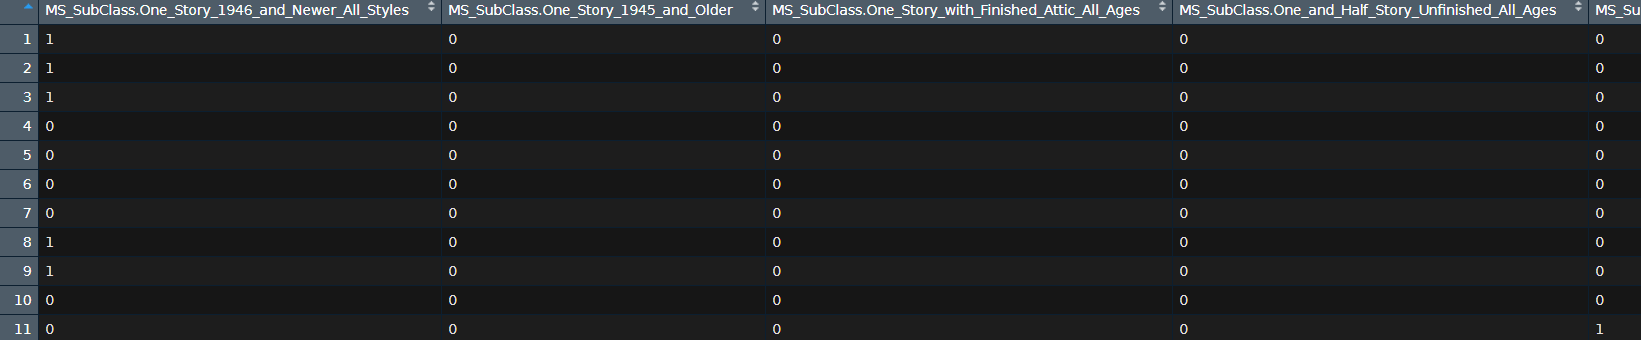
\includegraphics{figure/OneHotEncoding.PNG}

\end{frame}

\begin{frame}[fragile]{Hot encoding and hypergrid}
\protect\hypertarget{hot-encoding-and-hypergrid}{}

\begin{Shaded}
\begin{Highlighting}[]
\CommentTok{# make ranger compatible names}
\KeywordTok{names}\NormalTok{(ames_train_hot) <-}\StringTok{ }\KeywordTok{make.names}\NormalTok{(}\KeywordTok{names}\NormalTok{(ames_train_hot), }
                                    \DataTypeTok{allow_ =} \OtherTok{FALSE}\NormalTok{)}
\CommentTok{# --> same as above but with increased mtry values}
\NormalTok{hyper_grid_}\DecValTok{2}\NormalTok{ <-}\StringTok{ }\KeywordTok{expand.grid}\NormalTok{(}
  \DataTypeTok{mtry       =} \KeywordTok{seq}\NormalTok{(}\DecValTok{50}\NormalTok{, }\DecValTok{200}\NormalTok{, }\DataTypeTok{by =} \DecValTok{25}\NormalTok{),}
  \DataTypeTok{node_size  =} \KeywordTok{seq}\NormalTok{(}\DecValTok{3}\NormalTok{, }\DecValTok{9}\NormalTok{, }\DataTypeTok{by =} \DecValTok{2}\NormalTok{),}
  \DataTypeTok{sampe_size =} \KeywordTok{c}\NormalTok{(.}\DecValTok{55}\NormalTok{, }\FloatTok{.632}\NormalTok{, }\FloatTok{.70}\NormalTok{, }\FloatTok{.80}\NormalTok{),}
  \DataTypeTok{OOB_RMSE  =} \DecValTok{0}
\NormalTok{)}
\end{Highlighting}
\end{Shaded}

\end{frame}

\begin{frame}[fragile]{The best model}
\protect\hypertarget{the-best-model}{}

\begin{block}{The best random forest model:}

\begin{itemize}
\tightlist
\item
  uses columnar categorical variables
\item
  \texttt{mtry} = 24,
\item
  terminal node size of 5 observations
\item
  sample size of 80\%.
\end{itemize}

\end{block}

\begin{block}{How to proceed}

\begin{itemize}
\tightlist
\item
  Repeat the model to get a better expectation of error rate.
\end{itemize}

\end{block}

\end{frame}

\begin{frame}[fragile]{Random forests with \texttt{ranger}}
\protect\hypertarget{random-forests-with-ranger}{}

\begin{itemize}
\tightlist
\item
  The \texttt{impurity} measure is the variance of the responses for
  regression
\item
  \texttt{impurity} is a measure for heterogeneity - it measures how
  well the classes are\\
\end{itemize}

\begin{Shaded}
\begin{Highlighting}[]
\NormalTok{OOB_RMSE <-}\StringTok{ }\KeywordTok{vector}\NormalTok{(}\DataTypeTok{mode =} \StringTok{"numeric"}\NormalTok{, }\DataTypeTok{length =} \DecValTok{100}\NormalTok{)}
\ControlFlowTok{for}\NormalTok{(i }\ControlFlowTok{in} \KeywordTok{seq_along}\NormalTok{(OOB_RMSE)) \{}
\NormalTok{  optimal_ranger <-}\StringTok{ }\KeywordTok{ranger}\NormalTok{(}\DataTypeTok{formula=}\NormalTok{ Sale_Price }\OperatorTok{~}\StringTok{ }\NormalTok{., }
    \DataTypeTok{data            =}\NormalTok{ ames_train, }
    \DataTypeTok{num.trees       =} \DecValTok{500}\NormalTok{,}
    \DataTypeTok{mtry            =} \DecValTok{24}\NormalTok{,}
    \DataTypeTok{min.node.size   =} \DecValTok{5}\NormalTok{,}
    \DataTypeTok{sample.fraction =} \FloatTok{.8}\NormalTok{,}
    \DataTypeTok{importance      =} \StringTok{'impurity'}\NormalTok{)}
\NormalTok{  OOB_RMSE[i] <-}\StringTok{ }\KeywordTok{sqrt}\NormalTok{(optimal_ranger}\OperatorTok{$}\NormalTok{prediction.error)}
\NormalTok{\}}
\end{Highlighting}
\end{Shaded}

\end{frame}

\begin{frame}[fragile]{Variable importance / node impurity}
\protect\hypertarget{variable-importance-node-impurity}{}

\begin{itemize}
\item
  \href{https://stats.stackexchange.com/questions/223109/what-do-we-mean-by-node-impurity-ref-random-forest}{\textbf{Node
  impurity}} represents how well the trees split the data. There are
  several impurity measures;
\item
  Gini index, Entropy and misclassification error are
  \href{https://www.cs.indiana.edu/~predrag/classes/2017fallb365/ch4.pdf}{options}
  to measure the node impurity
\item
  We set
  \texttt{importance\ =\ \textquotesingle{}impurity\textquotesingle{}},
  which allows us to assess variable importance.
\item
  \href{https://topepo.github.io/caret/variable-importance.html}{\textbf{Variable
  importance}} is measured by recording the decrease in MSE each time a
  variable is used as a node split in a tree.
\item
  The remaining error left in predictive accuracy after a node split is
  known as node impurity. 
\item
  A variable that reduces this impurity is considered more imporant than
  those variables that do not.
\item
  We accumulate the reduction in MSE for each variable across all the
  trees and the variable with the greatest accumulated impact is
  considered the more important.
\end{itemize}

\end{frame}

\begin{frame}[fragile]{Plot the variable importance}
\protect\hypertarget{plot-the-variable-importance}{}

\begin{Shaded}
\begin{Highlighting}[]
\NormalTok{varimp_ranger <-}\StringTok{ }\NormalTok{optimal_ranger}\OperatorTok{$}\NormalTok{variable.importance }
\end{Highlighting}
\end{Shaded}

\begin{Shaded}
\begin{Highlighting}[]
\NormalTok{lattice}\OperatorTok{::}\KeywordTok{barchart}\NormalTok{(}\KeywordTok{sort}\NormalTok{(varimp_ranger)[}\DecValTok{1}\OperatorTok{:}\DecValTok{25}\NormalTok{],}\DataTypeTok{col=}\StringTok{"royalblue"}\NormalTok{)}
\end{Highlighting}
\end{Shaded}

\begin{itemize}
\tightlist
\item
  We see that Utilities has the greatest impact in reducing MSE across
  our trees, followed by \texttt{names(sort(varimp\_ranger)){[}2{]}},
  Low\_Qual\_Fin\_SF, etc.
\end{itemize}

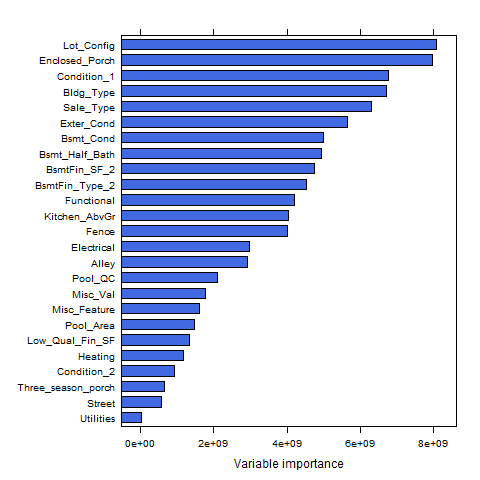
\includegraphics[width=\textwidth,height=0.6\textheight]{figure/ml_rf_varimp_ranger.png}

\end{frame}

\begin{frame}[fragile]{A histogram of OOB RMSE}
\protect\hypertarget{a-histogram-of-oob-rmse}{}

\begin{Shaded}
\begin{Highlighting}[]
\KeywordTok{hist}\NormalTok{(OOB_RMSE, }\DataTypeTok{breaks =} \DecValTok{20}\NormalTok{,}\DataTypeTok{col=}\StringTok{"royalblue"}\NormalTok{)}
\end{Highlighting}
\end{Shaded}

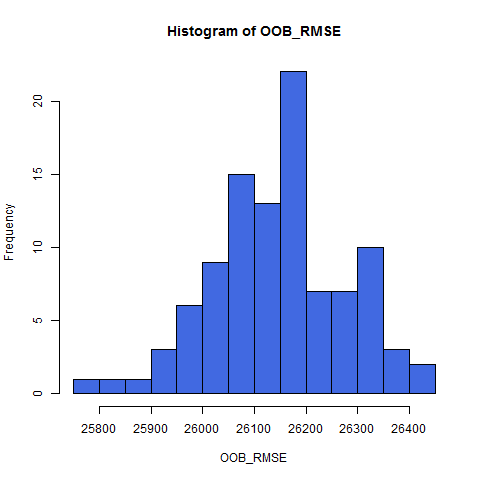
\includegraphics[width=\textwidth,height=0.75\textheight]{figure/ml_rf_hist_OOB_RMSE.png}

\end{frame}

\begin{frame}[fragile]{Predicting}
\protect\hypertarget{predicting}{}

\begin{itemize}
\tightlist
\item
  With the preferred model we can use the traditional predict function
  to make predictions on a new data set.
\item
  We can use this for all our model types (\texttt{randomForest} and
  \texttt{ranger}); although the outputs differ slightly. 
\end{itemize}

\begin{Shaded}
\begin{Highlighting}[]
\CommentTok{# randomForest}
\NormalTok{pred_randomForest <-}\StringTok{ }\KeywordTok{predict}\NormalTok{(ames_randomForest, ames_test)}
\KeywordTok{head}\NormalTok{(pred_randomForest)}
\end{Highlighting}
\end{Shaded}

\begin{verbatim}
##        1        2        3        4        5        6 
## 113543.1 185556.4 259258.1 190943.9 179071.0 480952.3
\end{verbatim}

\begin{Shaded}
\begin{Highlighting}[]
\CommentTok{# ranger}
\NormalTok{pred_ranger <-}\StringTok{ }\KeywordTok{predict}\NormalTok{(ames_ranger, ames_test)}
\KeywordTok{head}\NormalTok{(pred_ranger}\OperatorTok{$}\NormalTok{predictions)}
\end{Highlighting}
\end{Shaded}

\begin{verbatim}
## [1] 129258.1 186520.7 265628.2 197745.5 175517.6 392691.7
\end{verbatim}

\end{frame}

\begin{frame}{Summary - random forests}
\protect\hypertarget{summary---random-forests}{}

\begin{itemize}
\tightlist
\item
  Random forests provide a very powerful out-of-the-box algorithm that
  often has great predictive accuracy.
\item
  Because of their more simplistic tuning nature and the fact that they
  require very little, if any, feature pre-processing they are often one
  of the first go-to algorithms when facing a predictive modeling
  problem.
\end{itemize}

\end{frame}

\begin{frame}{Advantages \& Disadvantages}
\protect\hypertarget{advantages-disadvantages}{}

\begin{block}{Advantages - random forrests}

\begin{itemize}
\tightlist
\item
  Typically have very good performance
\item
  Remarkably good ``out-of-the box'' - very little tuning required
\item
  Built-in validation set - don't need to sacrifice data for extra
  validation
\item
  No pre-processing required
\item
  Robust to outliers
\end{itemize}

\end{block}

\begin{block}{Disadvantages - random forrests}

\begin{itemize}
\tightlist
\item
  Can become slow on large data sets
\item
  Although accurate, often cannot compete with advanced boosting
  algorithms
\item
  Less interpretable
\end{itemize}

\end{block}

\end{frame}

\begin{frame}{Links}
\protect\hypertarget{links}{}

These slides are mainly based on

\begin{itemize}
\item
  A UC Business Analytics R Programming Guide - section
  \href{http://uc-r.github.io/random_forests}{\textbf{random forests}}
\item
  and on the
  \href{https://bradleyboehmke.github.io/HOML/random-forest.html}{\textbf{chapter
  on random forests}} in the e-book of Brad Boehmke and Brandon
  Greenwell - Hands-on Machine Learning with R
\item
  \href{https://rpubs.com/nuhorchak/randomForest}{\textbf{Rpubs
  tutorial} - random forests}
\item
  \href{https://rpubs.com/anish20/RandomForests}{Random Forests in R}
\item
  \href{https://rpubs.com/Hgoswami/368562}{Boston Dataset-Tree Family
  Part-1}
\end{itemize}

\end{frame}

\end{document}
